\documentclass[../../notes.tex]{subfiles}

\pagestyle{main}
\renewcommand{\chaptermark}[1]{\markboth{\chaptername\ \thechapter\ (#1)}{}}
\setcounter{chapter}{2}

\begin{document}




\chapter{Determinants}
\begin{itemize}
    \item \marginnote{9/29:}The determinant, geometrically, is the volume of the object (in $\R^3$) you get when you take linear combinations of the vectors.
    \item In 2D:
    \begin{itemize}
        \item Let $v_1,v_2$ be two vectors. Put tail to tail and forming a parallelogram, the determinant of the matrix $(v_1,v_2)$ is the area of said parallelogram.
        \item Linearity 1: $D(av_1,v_2,\dots,v_n)=aD(v_1,\dots,v_n)$ is the same as saying that if you stretch one vector by $a$, you scale up the area by that much, too.
        \item Linearity 2: $D(v_1,\dots,v_{k+}+v_{k-},\dots,v_n)=D(-)+D(+)$.
        \item Antisymmetry: $D(v_1,\dots,v_k,\dots,v_j,\dots,v_n)=-D(v_1,\dots,v_j,\dots,v_k,\dots,v_n)$. Interchanging columns flips the sign of the determinant.
        \item Basis: $D(e_1,\dots,e_n)=1$.
    \end{itemize}
    \item Determinant: Denoted by $D(v_1,\dots,v_n)$, where $(v_1,\dots,v_n)$ is an $n\times n$ matrix.
    \item \marginnote{10/1:}Consider an $n\times n$ matrix $A$ consisting of $n$ columns containing vectors $\vm_1,\dots,\vm_n\in\R^n$.
    \begin{itemize}
        \item $D(A)$ is the volume of the solid $V=\sum_{i=1}^n\alpha_iv_i$.
        \item $D(\eb_1,\dots,\eb_n)=1$.
    \end{itemize}
    \begin{figure}[h!]
        \centering
        \footnotesize
        \begin{subfigure}[b]{0.45\linewidth}
            \centering
            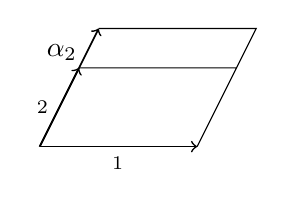
\begin{tikzpicture}
                \draw [semithick,->] (0,0) -- node[below]{$\vm_1$} (2,0);
                \draw [semithick,->] (0,0) -- node[left]{$\vm_2$} (0.5,1);
                \draw [semithick,->] (0,0) -- node[pos=0.8,left]{$\alpha\vm_2$} (0.75,1.5);
    
                \draw
                    (0.5,1)    -- ++(2,0) -- ++(-0.5,-1)
                    (0.75,1.5) -- ++(2,0) -- ++(-0.25,-0.5)
                ;
            \end{tikzpicture}
            \caption{$D(\vm_1,\alpha\vm_2)=\alpha D(\vm_1,\vm_2)$.}
            \label{fig:determinantPropertiesa}
        \end{subfigure}
        \begin{subfigure}[b]{0.45\linewidth}
            \centering
            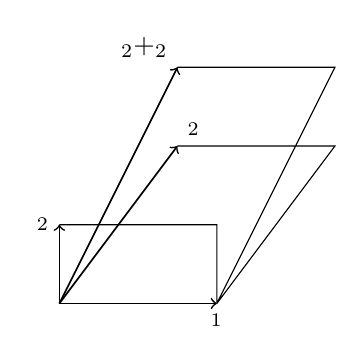
\begin{tikzpicture}
                \draw [semithick,->] (0,0) -- (2,0) node[below]{$\vm_1$};
                \draw [semithick,->] (0,0) -- (0,1) node[left]{$\vm_2$};
                \draw [semithick,->] (0,0) -- (1.5,2) node[above right]{$\wm_2$};
                \draw [semithick,->] (0,0) -- (1.5,3) node[above left]{$\vm_2+\wm_2$};
    
                \draw
                    (0,1) -- ++(2,0) -- ++(0,-1)
                    (1.5,2) -- ++(2,0) -- ++(-1.5,-2)
                    (1.5,3) -- ++(2,0) -- ++(-1.5,-3)
                ;
            \end{tikzpicture}
            \caption{$D(\vm_1,\vm_2+\wm_2)=D(\vm_1,\vm_2)+D(\vm_1,\wm_2)$.}
            \label{fig:determinantPropertiesb}
        \end{subfigure}
        \caption{Visualizing properties of determinants.}
        \label{fig:determinantProperties}
    \end{figure}
    \item Basic properties of the determinant.
    \begin{itemize}
        \item If $A$ has a zero column, then $\det A=0$: Scalar property.
        \item If $A$ has two equal columns, then $\det A=0$: Multiply one by minus and add.
        \item If $A$ has a column which is a multiple of another, then $\det A=0$: Pull out the multiple and then you have the previous one.
        \item If columns are linearly dependent, then $\det A=0$: Decompose it into sums, split, add back up with previous properties.
        \item The determinant is preserved under column reduction.
        \item $\det A^T=\det A$: Put everything in rref.
        \item If $A$ is not invertible, then $\det A=0$ (not invertible implies linearly dependent columns, implies $\det A=0$).
        \item $\det(AB)=\det A\det B$.
    \end{itemize}
    \item Determinant of\dots
    \begin{itemize}
        \item A diagonal matrix: The product of the diagonal entries (pull out the terms, and then note that the remaining identity matrix has determinant 1).
        \item An upper triangular matrix: The product of the diagonal entries (column reduction to make it into a diagonal matrix, and then the property above).
    \end{itemize}
\end{itemize}




\end{document}